\documentclass{beamer}

\mode<presentation> {
\usetheme{Madrid} }

\usepackage{graphicx} 
\usepackage{booktabs}
\usepackage[utf8]{inputenc}
\graphicspath{ {images/} }


%---Title Page---

\title[DP in Football]{Play Selection in American Football} 
\author[]{Daniel Bestard, Hans-Peter Hoellwirth, Akhil Lohia, Michael Cameron}
\institute[BGSE]{Barcelona Graduate School of Economics} 
\date{\today}

\begin{document}

\frame{\titlepage}

\begin{frame}
\frametitle{Motivation}
\begin{itemize}
\item Subconsciously, sport players compute probabilities
\pause
\item They use estimates of distances, angles and probabilities of events occurring
\pause
\item Aim: provide a framework for optimising decisions in American football
\pause
\item Use of DP to come up with the optimal policies. Two different implementations:
\pause
\begin{itemize}
\item Exact solution is feasible under some assumptions
\pause
\item For more general cases, approximations of the expected reward-to-go function are provided (API and OPI)
\end{itemize}
\end{itemize}
\end{frame}

\section{The Football Model}
\begin{frame}
\frametitle{Parameters of the dynamic programming algorithm}

\begin{itemize}
\item State of the system:
\begin{itemize}
\item $x_{i}$: yards to the goal line
\item $y_{i}$: yards to the first down
\item $d$: number of downs
\end{itemize}
\pause
\item Policies or actions that players can take:
\begin{itemize}
\item P: pass
\item R: run
\item U: punt
\item K: kick
\end{itemize}
\pause
\item Rewards:
\begin{itemize}
\item Touchdown: $6.8$
\item Field goal: $3$
\item Safety: $-2$
\item Opposition score = $ -\frac{6.8 x}{100}$
\end{itemize}
\end{itemize}
\end{frame}

\begin{frame}
\frametitle{Exact Dynamic Programming}
\begin{block}{DP Equation}
\begin{center}
$\mu^{k}(i) = arg\max\limits_{u \in U} \Big[ \sum\limits_{j \in S} p_{ij}(u)(g(i,u,j) +  J^{\mu^{k-1}}(j))\Big] \, \, \, \forall i \in S$
\end{center}
\end{block}
\begin{itemize}
\item $p_{ij}(u)$: transition probabilities
\item $g(i,u,j)$: reward function
\item $J^{\mu^{k-1}}(j)$: reward-to-go function
\end{itemize}
$J$ is computed exactly using the 15250 possible states of the system.
\end{frame}

\begin{frame}
\frametitle{Simulations}
\begin{itemize}
\item We create a reasonable class of policies and implement it. 
\item Policies are compared by calculating the points from one drive.
\item Simulations for an optimal heuristic policy are run from the starting state of $(x_{i},y_{i},d) = (80, 10, 1)$.
\item Example of a simulation:
\end{itemize}
$$
\begin{bmatrix} 25\\[0.3em] 10 \\[0.3em] 1 \end{bmatrix}
\longrightarrow_0^P
\begin{bmatrix} 17\\[0.3em] 2 \\[0.3em] 2 \end{bmatrix}
\longrightarrow_0^R
\begin{bmatrix} 14\\[0.3em] 10 \\[0.3em] 1 \end{bmatrix}
\longrightarrow_0^P
\begin{bmatrix} 10\\[0.3em] 6 \\[0.3em] 2 \end{bmatrix}
\longrightarrow_0^P
\begin{bmatrix} 10\\[0.3em] 6 \\[0.3em] 3 \end{bmatrix}
\longrightarrow_0^R
\begin{bmatrix} 8\\[0.3em] 4 \\[0.3em] 4 \end{bmatrix}
\longrightarrow_3^K
T
$$
\end{frame}

\begin{frame}
\frametitle{Policy Update}
\begin{block}{Approximated DP algorithm}
\begin{center}
$\mu^{k}(i) = arg\max\limits_{u \in U} \Big[ \sum\limits_{j \in S} p_{ij}(u)(g(i,u,j) +  \widetilde{J}^{\mu^{k-1}}(j))\Big]$
\end{center}
\end{block}
\end{frame}

\begin{frame}
\frametitle{API and OPI Algorithm}
\begin{itemize}
\item Algorithm:
\begin{enumerate}
\item Start an initial policy $\mu_{0}$
\item For each $k \in \{1,\ldots, K\}$ :
\begin{enumerate}
\item Given $\mu_{k-1}$, simulate $N_{s}$ sample trajectories
\item Fit the neural network using the sample data to estimate the $J^{\mu^{k-1}}$
\item Update policy to get $\mu^{k}$
\end{enumerate}
\end{enumerate}
\item Two different ways to make the approximations
\begin{itemize}
\item API: Many training sample points, few iterations
\item OPI: Few training sample points, many iterations
\end{itemize}
\end{itemize}

\end{frame}

\begin{frame}
\frametitle{Neural Network}
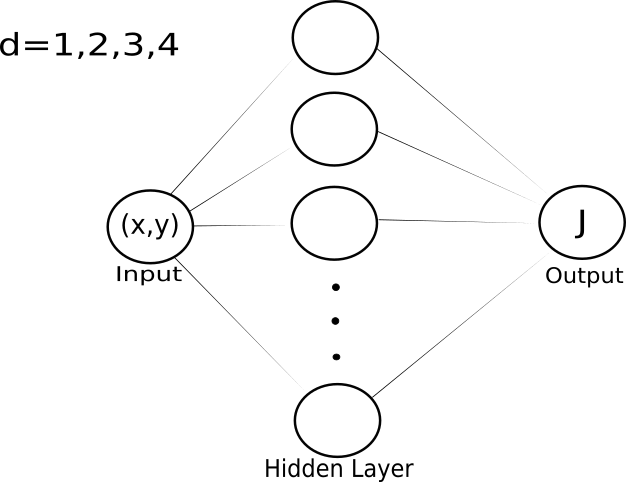
\includegraphics[scale=0.65]{neuralnet}
\end{frame}

\begin{frame}
\frametitle{Super Bowl XLIX}
\begin{center}
Seahawks should have run!
\end{center}
\end{frame}
\end{document}